% !TEX root = ../YourName-Dissertation.tex
\Appendix{Supportive Data and Figures}

\section{Data}
% Table generated by Excel2LaTeX from sheet 'Sheet1'
\begin{table}[htbp]
  \centering
  \caption{Data Source and operation for the empirical test in Section 2.3.3}
  \begin{tabular}{ccp{8.785em}c}
    \toprule
    \multicolumn{2}{p{13.93em}}{Variables }                                         & Source  & \multicolumn{1}{p{7.785em}}{Time Period}                                                                         \\
    \midrule
    \multicolumn{1}{p{7em}}{Dependent Variable}                                     & lg(igt) & State CAFR                               & \multicolumn{1}{c}{\multirow{9}[18]{*}{2000-2019 annually collected}} \\
    \cmidrule{1-3}    \multicolumn{1}{c}{\multirow{2}[4]{*}{Independent Variables}} & c       & \multirow{2}[4]{*}{Ballotpedia}          &                                                                       \\
    \cmidrule{2-2}                                                                  & p       & \multicolumn{1}{c}{}                     &                                                                       \\
    \cmidrule{1-3}    \multicolumn{1}{c}{\multirow{6}[12]{*}{Control Variables}}    & gdp     & FRED                                     &                                                                       \\
    \cmidrule{2-3}                                                                  & lgp     & \multirow{4}[8]{*}{Census of bureau}     &                                                                       \\
    \cmidrule{2-2}                                                                  & wapw    & \multicolumn{1}{c}{}                     &                                                                       \\
    \cmidrule{2-2}                                                                  & mhi     & \multicolumn{1}{c}{}                     &                                                                       \\
    \cmidrule{2-2}                                                                  & ur      & \multicolumn{1}{c}{}                     &                                                                       \\
    \cmidrule{2-3}                                                                  & prm     & Bureau of transportation statistics      &                                                                       \\
    \bottomrule
  \end{tabular}%
  \label{Table A.1}%
\end{table}%


\section{Figures}
%%%
%%%%%%%%%%%%%%%%%%%%%%%%%%%%%%%%%%
\begin{figure}[H]
  \centering  %居中
  \subfigure[Federal Expenditure]{   %first subfigure
    \begin{minipage}{7cm}
      \centering    %子图居中
      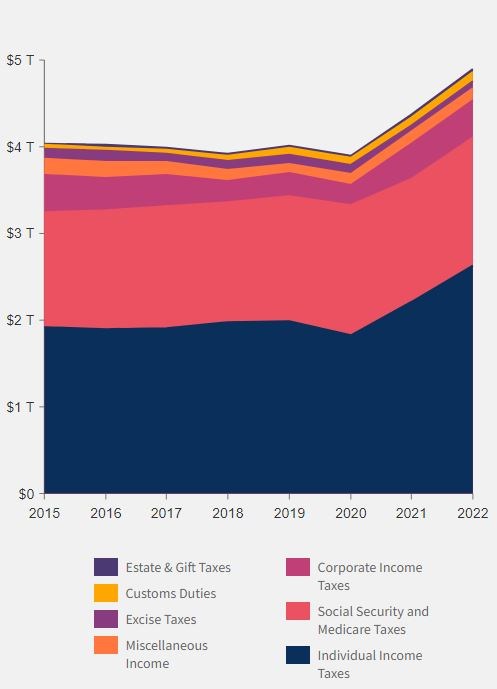
\includegraphics[scale=0.52]{Chapter-1/Figures/source of federal revenue.JPG}  %以pic.jpg的0.5倍大小输出
    \end{minipage}
  }
  \subfigure[State and Local Expenditure]{ %second subfigure
    \begin{minipage}{7cm}
      \centering    %子图居中
      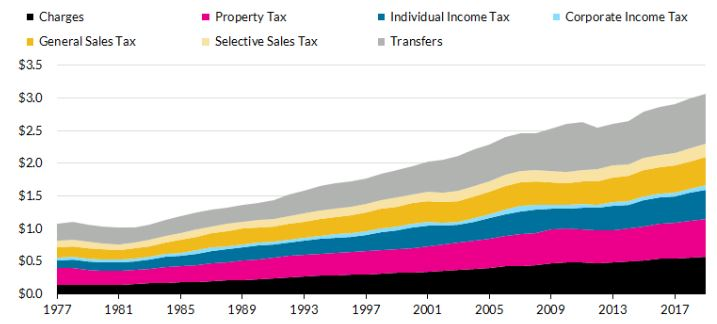
\includegraphics[scale=0.52]{Chapter-1/Figures/source of state and local revenue.JPG}%以pic.jpg的0.5倍大小输出
    \end{minipage}
  }

  \caption[Fluctuation of Revenue Structure]{Fluctuation of Revenue Structure of three level governments.Data Source: US Urban Institute Dataset  }    %caption for whole figure
  \label{Figure A.1}
\end{figure}

%%%%%%%%%%%%%%%%%%%%%%%%%%%%%%%%%%%%%%%%%%%%%%%

\begin{figure}[H]
  \centering
  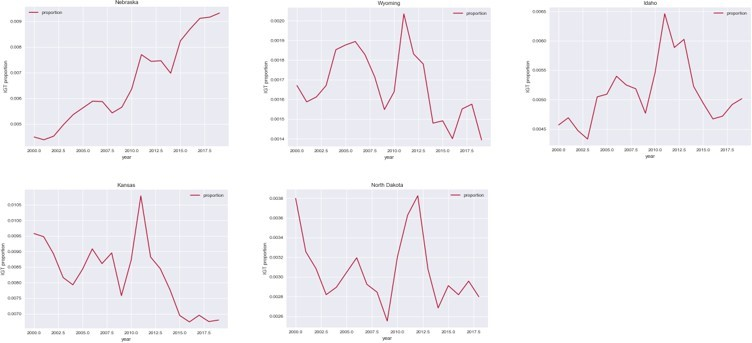
\includegraphics[scale=0.7]{Appendix-A/republican.jpg}
  \caption[Time Series Graph of Republican States IGT (2000-2019)]{Time Series Graph of Republican States IGT (2000-2019)
    \texttt{} }
  \label{Figure A.2}
\end{figure}

\begin{figure}[H]
  \centering
  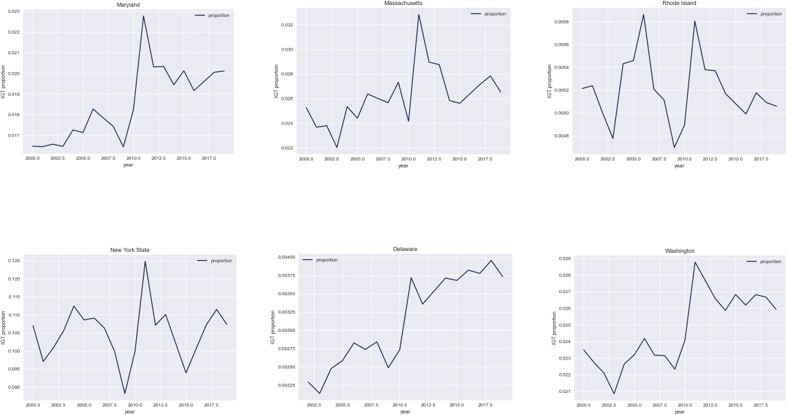
\includegraphics[scale=0.7]{Appendix-A/democratic.jpg}
  \caption[Time Series Graph of Democratic States IGT(2000-2019)]{Time Series Graph of Democratic States IGT (2000-2019)
    \texttt{} }
  \label{Figure A.3}
\end{figure}

\begin{figure}[H]
  \centering
  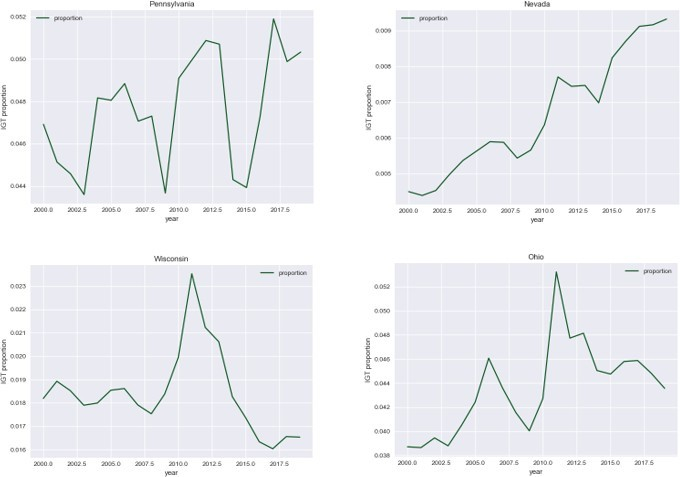
\includegraphics[scale=0.7]{Appendix-A/swing.jpg}
  \caption[Time Series Graph of Swing States IGT (2000-2019) ]{Time Series Graph of Swing States IGT (2000-2019)
    \texttt{} }
  \label{Figure A.4}
\end{figure}
